\chapter{Extending GDB for \uCPP}

\section{Introduction}
A sequential program has a single call stack. A debugger knows about this call
stack and provides commands to walk up/down the call frames to examine the
values of local variables, as well as global variables. A concurrent program
has multiple call stacks (for coroutines/tasks), so a debugger must be extended
to locate these stacks for examination, similar to a sequential stack.  For
example, when a concurrent program deadlocks, looking at the task's call stack
can locate the resource and the blocking cycle that resulted in the
deadlock. Hence, it is very useful to display the call stack of each task to
know where it is executing and what values it is currently computing. Because
each programming language's concurrency is different, GDB has to be
specifically extended for \uCPP.

\section{Design Constraints}
As mentioned in Chapter \ref{GDB}, there are several ways to extend GDB. However,
there are a few design constraints on the selected mechanism. All the functions
implemented should maintain similar functionality to existing GDB commands. In addition to functional
requirements, usability and flexibility are requirements for this
project. These final requirements enable developers to be productive quickly
and do more with the extensions. The extensions created for \uCPPS are simple
to use and versatile.

The following new GDB command are all implemented through the Python API for
GDB.  Python is a scripting language with built-in data structures and
functions that enables the development of more complex operations and saves
time on development.

\section{\uCPPS source-code example}
Listing \ref{uCPP-src-code} shows a \uCPPS program that implicitly creates two
clusters, system and user, which implicitly have a processor (kernel thread)
and processor task. The program explicitly creates three additional processors
and ten tasks on the user cluster.

\begin{figure}
\begin{lstlisting}[style=C++, caption={\uCPPS source code used for GDB commands},
label={uCPP-src-code}, basicstyle=\small]
_Task T {
    std::string name;

    void a(int param) {
        if ( param != 0 ) a( param - 1 );
        int x = 3;
        std::string y = "example";
    }
    void main() {
        a(3);
    }
  public:
    T(const int tid) {
        name = "T" + std::to_string(tid);
        setName(tid.c_str());
    }
};

int main() {
    uProcessor procs[3];	// extra processors
    const int numTasks = 10;
    T* tasks[numTasks];		// extra tasks

    // allocate tasks with different names
    for (int id = 0; id < numTasks; id += 1) {
        tasks[i] = new T(id);
    }
    // deallocate tasks
    for (int id = 0; id < numTasks; id += 1) {
        delete tasks[i];
    }
}
\end{lstlisting}
\end{figure}

\section{Existing User-defined GDB Commands}
Listing \ref{uCPP-callstack} shows the GDB output at the base case of the
recursion for one of the tasks created in the \uCPPS program in listing
\ref{uCPP-src-code}.  The task is stopped at line 8. The backtrace shows the
three calls to function \verb|a|, started in the task's \verb|main|. The top
two frames are administrative frames from \uCPP. The values of the argument and
local variables are printed.

\begin{figure}
\begin{lstlisting}[caption={Call stack of function \texttt{a} in the \uCPPS
program from listing \ref{uCPP-src-code}}, label={uCPP-callstack}, basicstyle=\small\tt]
(gdb) backtrace
#0  T::a (this=0x907880, param=0) at test.cc:8
#1  0x000000000041d207 in T::a(this=0x907880, param=1) at test.cc:5
#2  0x000000000041d207 in T::a(this=0x907880, param=2) at test.cc:5
#3  0x000000000041d207 in T::a(this=0x907880, param=3) at test.cc:5
#4  0x000000000041d2c0 in T::main(this=0x907880) at test.cc:10
#5  0x000000000042633f in ...::invokeTask(uBaseTask&) at ...
#6  0x0000000000000000 in ?? ()
(gdb) info args
this = 0x907880
param = 0
(gdb) info locals
x = 3
y = "example"
\end{lstlisting}
\end{figure}

\subsection{Listing all clusters in a \uCPPS program}
Listing \ref{clusters-command} shows the new command \verb|clusters| to list
all program clusters along with their associated address.  The output shows the
two \uCPPS implicitly created clusters.
\begin{figure}
\begin{lstlisting}[caption={clusters command}, label={clusters-command}, basicstyle=\small\tt]
(gdb) clusters
        Name            Address
    systemCluster       0x655280
    userCluster         0x7c4280
\end{lstlisting}
\end{figure}

\subsection{Listing all processors in a cluster}
Listing \ref{cluster-procs} shows the new command \verb|processors|, which
requires a cluster argument to show all the processors in that cluster. In
particular, this example shows that there are four processors in the
\verb|userCluster|, with their associated address, PID, preemption and spin.
\begin{figure}
\begin{lstlisting}[caption={processors command}, label={cluster-procs}, basicstyle=\small\tt]
(gdb) processors userCluster
    Address    PID         Preemption      Spin
    0x7c6bf0    8396928     10              1000
    0x8c3b60    9453696     10              1000
    0x8c3d20    9977984     10              1000
    0x8c3ee0    10506368    10              1000
\end{lstlisting}
\end{figure}

\subsection{Listing all tasks in all clusters}
Listing \ref{tasks} shows the new command \verb|task| without an argument to
list all the tasks in a \uCPPS program at this point in the execution snapshot.
\begin{figure}
\begin{lstlisting}[caption={task command for displaying all tasks for all
clusters}, label={tasks}, basicstyle=\small\tt]
(gdb) task
        Cluster Name        Address
        systemCluster       0x655280
    ID      Task Name            Address         State
    0       uProcessorTask      0x6c39b0        uBaseTask::Blocked
    1       uSystemTask         0x783ef0        uBaseTask::Blocked
        Cluster Name        Address
        userCluster         0x7c4280
    ID      Task Name            Address         State
    0       uProcessorTask      0x806e70        uBaseTask::Blocked
    ...
    6       T0                  0xa49830        uBaseTask::Ready
    7       T1                  0xa89bb0        uBaseTask::Running
    8       T2                  0xac9f30        uBaseTask::Ready
    ...
    15      T9                  0xc8b7b0        uBaseTask::Ready
\end{lstlisting}
\end{figure}

\subsection{Listing all tasks in a cluster}
Listing \ref{cluster-tasks} shows the new command \verb|task| with a cluster
argument to list only the names of the tasks on that cluster.  In this version
of the command \verb|task|, the associated address for each task and its state
is displayed.
\begin{figure}
\begin{lstlisting}[caption={task command for displaying all tasks in a cluster}, label={cluster-tasks}, basicstyle=\small\tt]
(gdb) task systemCluster
    ID          Name            Address         State
    0       uProcessorTask      0x654200        uBaseTask::Blocked
    1       uSystemTask         0x7c3280        uBaseTask::Blocked
\end{lstlisting}
\end{figure}

\section{Changing Stacks}
The next extension for displaying information is writing new commands that allow
stepping from one \uCPPS task to another. Two switching approaches are
provided: structured and free form. The structured form remembers the task tour in a
LIFO way, while the free form does not remember the task tour. This semantics means
at least two commands are needed for the structured form and the free form.
Taking the idea of overloading in programming languages, the structured
commands for switching from the current task to a different task overload the
command \verb|task| with two arguments, and
for switching back to the previous task is a new command \verb|poptask|.

\subsection{Task Switching}
Both overloaded \verb|task| or \verb|poptask| commands allow two ways to
designate a task: its absolute address or relative id within a cluster. For
instance, to switch from any task to task \verb|T1| seen in listing
\ref{tasks}, the first command in listing \ref{task-addr-option} uses an
absolute address (0xa49830) and the second command uses a relative id (6) with
respect to userCluster. Core functionality of these approaches is essentially the same.
\begin{lstlisting}[caption={task command option}, label={task-addr-option}, basicstyle=\small\tt]
task 0xa49830
task userCluster 6
\end{lstlisting}

\subsection{Switching Implementation}
To implement the task tour, it is necessary to store the context information
for every context switching. This requirement means the \verb|task| command
needs to store this information every time it is
invoked.

Figure \ref{machine-context} shows a task points to a structure containing a
\verb|uContext_t| data structure, storing the stack and frame pointer, and the
stack pointer. Listing \ref{pushtask-code} shows these pointers are copied into
an instance of the Python tuple \verb|StackInfo| for every level of task
switching. This tuple also stores information about the program counter that is
calculated from the address of the \verb|uSwitch| Assembly function because a
task always stops in \verb|uSwitch| when its state is blocked.  Similarly,
switching commands retrieve this context information but from the task that
a user wants to switch to, and sets the equivalent registers to the new values.

\begin{figure}[h]
    \centering
    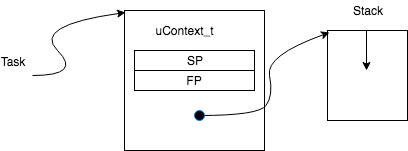
\includegraphics[width=8cm]{uContext_stack}
    \caption{Machine context (uMachContext) for each task}
    \label{machine-context}
\end{figure}

For free-form touring using the \verb|task| command, the value of the stack
pointer is copied to/from the \verb|rsp| register, the value of the frame
pointer is copied to/from the \verb|rbp| register, and finally the value of the
program counter is copied to/from the \verb|pc| register.

\begin{figure}
\begin{lstlisting}[style=Python, caption={Abridged \texttt{push\_task} source
code}, label={pushtask-code}, basicstyle=\small\tt]
# get GDB type of uContext_t*
uContext_t_ptr_type =
   gdb.lookup_type('UPP::uMachContext::uContext_t').pointer

# retrieve the context object from a task
# and cast it to the type uContext_t*
task_context = task['context'].cast(uContext_t_ptr_type)

# the offset where sp would be starting from uSwitch function
sp_address_offset = 48
# lookup the value of stack pointer (sp), frame pointer (fp),
# program counter (pc)
xsp = task_context['SP'] + sp_address_offset
xfp = task_context['FP']
if not gdb.lookup_symbol('uSwitch'):
    print('uSwitch symbol is not available')
    return

# This value is calculated here because we always here when
# the task is in blocked state
xpc = get_addr(gdb.parse_and_eval('uSwitch').address + 28, 'PC')
# must switch back to frame-0 to set 'pc' register with
# the value of xpc
gdb.execute('select-frame 0')

# retrieve register values and push sp, fp, pc into
# a global stack
global STACK
sp = gdb.parse_and_eval('$sp')
fp = gdb.parse_and_eval('$fp')
pc = gdb.parse_and_eval('$pc')
stack_info = StackInfo(sp = sp, fp = fp, pc = pc)
STACK.append(stack_info)

# update registers for a new task
gdb.execute('set $rsp={}'.format(xsp))
gdb.execute('set $rbp={}'.format(xfp))
gdb.execute('set $pc={}'.format(xpc))
\end{lstlisting}
\end{figure}

For structured touring, the implementation manages a stack of toured tasks.
The \verb|pushtask| command sets the appropriate registers to move to the
specified task, and remembers the previous task registers.  The \verb|poptask|
restores the previous stack register. Popping an empty stack prints a warning.
In particular, listing \ref{poptask} shows the backtrace after touring to task
6 of \verb|userCluster|, whose address can be seen on line 23. However, after
calling the command \verb|poptask|, the new backtrace shows the address of the
previous task, which is \verb|0xb0a2b0| and seen on lines 11 and 30.

\begin{figure}
\begin{lstlisting}[numbers=left, caption={\texttt{poptask} command}, label={poptask}, basicstyle=\footnotesize\tt]
(gdb) info threads
  Id   Target Id         Frame
* 1    Thread 0x7ffff7fe9780 (LWP 704) "utils" 0x000000000042f2ef in
        uCluster::processorPause (this=0x73f7a8) at
        /usr/local/u++-7.0.0/src/kernel/uCluster.cc:120
  2    Thread 0x802080 (LWP 708) "utils" T::a (this=0xa49830) at utils.cpp:7
  3    Thread 0x904080 (LWP 709) "utils" T::a (this=0xbcad30) at utils.cpp:7
  4    Thread 0x984080 (LWP 710) "utils" T::a (this=0xb8a9b0) at utils.cpp:7
  5    Thread 0xa05080 (LWP 711) "utils" UPP::uSigHandlerModule::sigAlrmHandler
        (sig=10, sfp=0xb864b0, cxt=0xb86380) at
        /usr/local/u++-7.0.0/src/kernel/uSignal.cc:218
(gdb) thread 2
(gdb) backtrace
<@\textcolor{ForestGreen}{\#0  T::a (this=0xb0a2b0, param=5) at utils.cpp:8}@>
#1  0x000000000041cb4c in T::main (this=0xb0a2b0) at
utils.cpp:11
#2  0x0000000000425bbc in UPP::uMachContext::invokeTask (This=...)
    at /usr/local/u++-7.0.0/src/kernel/uMachContext.cc:140
#3  0x0000000000000000 in ?? ()
(gdb) task userCluster 6
(gdb) backtrace
#0  uSwitch () at /usr/local/u++-7.0.0/src/kernel/uSwitch-x86_64.S:64
#1  0x00000000004288ec in uBaseCoroutine::taskCxtSw (this=0x8c3b78)
    at /usr/local/u++-7.0.0/src/kernel/uBaseCoroutine.cc:146
...
<@\textcolor{ForestGreen}{\#7  T::a (this=0xa49830) at utils.cpp:8}@>
#8  0x000000000041cb43 in T::main (this=0xa49830) at utils.cpp:11
#9  0x0000000000425bbc in UPP::uMachContext::invokeTask (This=...)
    at /usr/local/u++-7.0.0/src/kernel/uMachContext.cc:140
#10 0x0000000000000000 in ?? ()
(gdb) poptask
(gdb) backtrace
<@\textcolor{ForestGreen}{\#0  T::a (this=0xb0a2b0, param=5) at utils.cpp:8}@>
#1  0x000000000041cb4c in T::main (this=0xb0a2b0) at utils.cpp:11
#2  0x0000000000425bbc in UPP::uMachContext::invokeTask (This=...)
    at /usr/local/u++-7.0.0/src/kernel/uMachContext.cc:140
#3  0x0000000000000000 in ?? ()
\end{lstlisting}
\end{figure}

\subsection{Continuing Implementation}
When a breakpoint or error is encountered, all concurrent execution stops.  The
state of the program can now be examined and changed; after which the program
can be continued. Continuation must always occur from the top of the stack
(current call) for each task, and at the specific task where GDB stopped
execution.

However, during a task tour, the new GDB commands change the notion of the task
where execution stopped to make it possible to walk other stacks.  Hence, it is
a requirement for continuation that the task walk always return to frame-0 of
the original stopped task before any program continuation \cite{Reference11}.

% For every new function call, a new stack frame is created and the values of all
% the registers are changed for that frame. Therefore, in order to see the true
% value of hardware registers, innermost frame that is frame-0 must be selected
% \cite{Reference11}. However, it is possible to not be in frame-0, so prior to
% setting these values, the command must switch back to the innermost (currently
% executing) frame first.

To provide for this requirement, the original stop task is implicitly
remembered, and there is a new \verb|reset| command that \emph{must} be
explicitly executed before any continuation to restore the locate state.  To
prevent errors from forgetting to call the \verb|reset| command, additional
hooks are added to the existing built-in GDB continuation commands (see
\ref{continue-cmds}) to implicitly call \verb|reset|. The list of these
commands results from GDB documentation \cite{Reference15} and similar work
done for KOS \cite{Reference14}.

% These hooks call a new command called \verb|reset| prior to executing the
% command to enable continuation of a program to ensure that the program's
% context is automatically switched back to the context of the task that
% initiates the first context switch. The \verb|reset| command behaves as same as
% the command \verb|poptask|, however, it goes back directly to where the task is
% when the program last stops, which is the first task in the task tour.

\begin{figure}
\begin{lstlisting}[caption={Built-in GDB commands that allow continuation of a
program}, label={continue-cmds}, basicstyle=\small\tt]
continue
next
nexti
step
stepi
finish
advance
jump
signal
until
reverse-next
reverse-step
reverse-stepi
reverse-continue
reverse-finish
\end{lstlisting}
\end{figure}

\section{Result}
The current implementation successfully allows users to display a snapshot of
\uCPPS execution with respect to clusters, processors, and tasks. With this
information it is possible to tour the call stacks of the tasks to see
execution locations and data values. Additionally, users are allowed to
continue the execution where the program last pauses assuming that the program
has not crashed. The continuation of execution is done by automatically
reversing the task walk from any existing GDB commands such as \verb|continue|,
or a user can manually reverse the task walk using the command \verb|poptask|
and then continue.
